\documentclass[11pt]{article}
\usepackage[margin=1in]{geometry}
\usepackage{amsmath,amssymb,amsthm}
\usepackage{graphicx}
\usepackage[hidelinks]{hyperref}

\newtheorem{theorem}{Theorem}
\newtheorem{remark}{Remark}

\newcommand{\X}{\mathfrak X}
\newcommand{\N}{\mathfrak N}
\newcommand{\R}{\mathbb R}
\newcommand{\Span}{\operatorname{span}}
\newcommand{\Cb}{C_b}

\title{A Ray Obstruction to Global \(C_b\) Approximation for Rank-One Sigmoid Frechet Networks}
\author{FA Banach run \texttt{fa\_banach\_001}, agent \texttt{agent\_lane\_12}}
\date{2026-06-20}

\begin{document}
\maketitle

\section*{Status}

This packet records a candidate counterexample, likely valid. It disproves a
natural global supremum-norm strengthening of the rank-one sigmoid activation
example in Benth--Detering--Galimberti, arXiv:2109.13512v4. It does not
contradict their compact-open density theorem.

\section*{Source Passage}

Remark 2.2 of the source paper says that it would be tempting to work directly
in \(\Cb(\X;\mathbb F)\), endowed with the supremum norm, after imposing
boundedness assumptions on the nonlinearity \(\sigma\).

\begin{center}

\includegraphics[width=0.98\linewidth]{figures/open_problem_crop.png}
\end{center}

The activation class treated here is the source paper's one-coordinate sigmoid
example: after choosing \(\psi\in \X'\setminus\{0\}\), \(z\in \X\), and
\(\beta\in C(\R;\R)\) with
\[
  \lim_{\xi\to\infty}\beta(\xi)=1,\qquad
  \lim_{\xi\to-\infty}\beta(\xi)=0,\qquad
  \beta(0)=0,
\]
the source notes that
\[
  \sigma(x)=\beta(\psi(x))z
\]
still gives compact-open density in \(C(\X;\R)\).

\begin{center}
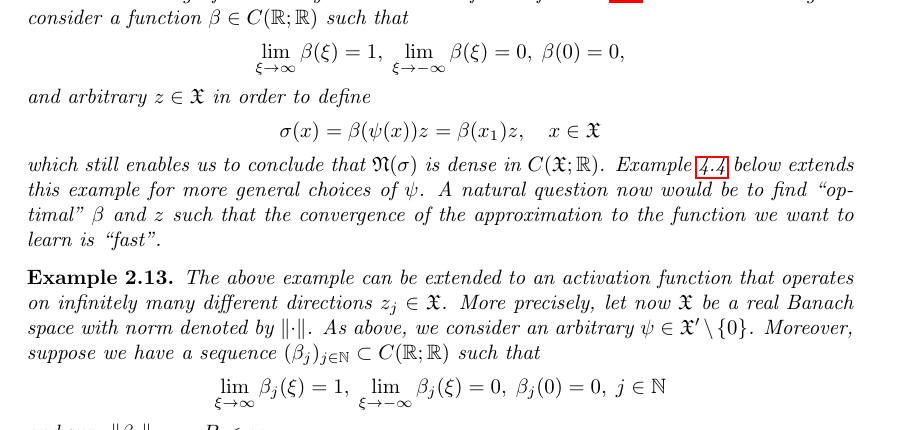
\includegraphics[width=0.98\linewidth]{figures/rank_one_sigmoid_example_crop.png}
\end{center}

\section*{Transcription of the Target}

The relevant part of Remark 2.2 reads, in substance: it would be interesting to
establish the universal approximation result in the global space of bounded
continuous functions \(\Cb(\X;\mathbb F)\), with the supremum norm, under
suitable boundedness assumptions on \(\sigma\). The authors identify the dual
space \(rba(\X)\) and finitely additive measures as the obstruction to a direct
Cybenko-type proof.

\section*{The Counterexample}

\begin{theorem}
Let \(\X\) be a nonzero real Frechet space. Let
\(\psi\in \X'\setminus\{0\}\), let \(z\in\X\setminus\{0\}\), and let
\(\beta\in C_b(\R)\) have finite one-sided limits
\[
  \beta(+\infty):=\lim_{s\to\infty}\beta(s),\qquad
  \beta(-\infty):=\lim_{s\to-\infty}\beta(s).
\]
Define
\[
  \sigma(x)=\beta(\psi(x))z,\qquad x\in\X,
\]
and let
\[
  \N(\sigma)=
  \Span\{x\mapsto \ell(\sigma(Ax+b)):
        \ell\in \X',\ A\in\mathcal L(\X),\ b\in\X\}.
\]
Then \(\N(\sigma)\) is not dense in \(\Cb(\X;\R)\) with the supremum norm.
Indeed, there is \(f\in\Cb(\X;\R)\) such that
\[
  \inf_{g\in \N(\sigma)}\|f-g\|_\infty \ge 1.
\]
\end{theorem}

\section*{Idea of the Proof}

The source's one-coordinate sigmoid activation collapses every neuron to a
bounded scalar sigmoid of one affine functional. Along any fixed ray
\(t\mapsto tv\), every such scalar input is affine in \(t\), so the finite
limits of \(\beta\) force every neuron, and hence every finite network, to have
a finite ray limit. But \(\Cb(\X)\) contains bounded continuous functions that
oscillate forever along the same ray, for example \(x\mapsto
\sin(\varphi(x)^2)\). Such a function cannot be uniformly approximated by
functions with a ray limit.

\section*{Proof}

\begin{proof}
Because \(\X\) is a nonzero Hausdorff locally convex space, its continuous
dual separates points. Choose \(v\in\X\) and \(\varphi\in\X'\) such that
\(\varphi(v)=1\). Set
\[
  f(x)=\sin(\varphi(x)^2),\qquad x\in\X.
\]
Then \(f\in \Cb(\X;\R)\).

Let \(h(x)=\ell(\sigma(Ax+b))\) be one neuron. Along the ray \(t\mapsto tv\),
\[
  h(tv)
  =\ell(z)\,\beta(\psi(A(tv)+b))
  =\ell(z)\,\beta(t\,\psi(Av)+\psi(b)).
\]
If \(\psi(Av)>0\), this tends to \(\ell(z)\beta(+\infty)\). If
\(\psi(Av)<0\), it tends to \(\ell(z)\beta(-\infty)\). If
\(\psi(Av)=0\), it is the constant \(\ell(z)\beta(\psi(b))\). Thus every
neuron has a finite limit along \(tv\) as \(t\to\infty\), and therefore every
finite linear combination \(g\in\N(\sigma)\) has a finite ray limit
\[
  L_g:=\lim_{t\to\infty}g(tv).
\]

On the other hand,
\[
  f(tv)=\sin(\varphi(tv)^2)=\sin(t^2).
\]
Let
\[
  t_n=\sqrt{\frac{\pi}{2}+2\pi n},
  \qquad
  s_n=\sqrt{\frac{3\pi}{2}+2\pi n}.
\]
Then \(t_n,s_n\to\infty\), while
\[
  f(t_n v)=1,\qquad f(s_n v)=-1.
\]
Suppose, for contradiction, that some \(g\in\N(\sigma)\) satisfies
\(\|f-g\|_\infty<\varepsilon\) for some \(\varepsilon<1\). Passing to the
limits along the two sequences gives
\[
  |1-L_g|\le \varepsilon,
  \qquad
  |-1-L_g|\le \varepsilon.
\]
Hence
\[
  2=|1-(-1)|\le |1-L_g|+|-1-L_g|\le 2\varepsilon<2,
\]
a contradiction. Therefore no \(g\in\N(\sigma)\) can approximate \(f\) within
supremum error \(<1\), and the distance from \(f\) to \(\N(\sigma)\) is at
least \(1\).
\end{proof}

\section*{Verification Notes}

The proof is purely analytic and uses no computation. The only topological
vector space fact used outside the source definitions is the standard
separation property of nonzero Hausdorff locally convex spaces: for a nonzero
point one can find a continuous linear functional not vanishing at that point.
This is a direct Hahn--Banach consequence.

The finite limits of \(\beta\) are exactly the needed input. Monotonicity,
sigmoid shape, and the normalization \(\beta(0)=0\) play no role in the
negative global result.

\section*{Novelty and Literature Check}

The run indexes were searched for arXiv:2109.13512, the source title,
``Frechet spaces'', ``Fr\'echet spaces'', ``neural'', ``\(C_b\)'',
``supremum norm'', ``finitely additive'', ``discriminatory'', and the formula
``sigma(x)=beta(psi(x))z''. No exact previous packet was found. One adjacent
run entry concerns arXiv:2105.02095 and a different Banach-valued neural
network question.

External web searches on 2026-06-20 used the source title together with
``\(C_b\)'', ``supremum norm'', ``finitely additive'', and ``discriminatory'',
plus targeted searches for ``sigma(x)=beta(psi(x)) z'', ``sigmoidal \(C_b\)
not dense'', and ``sin(x\^{}2)'' ray-obstruction language. These searches
returned the source arXiv page but no separate answer or matching
counterexample. Novelty confidence is moderate: the argument is short and may
be folklore in the classical \(C_b(\R^n)\) setting, but no source was found
that records this obstruction for the Frechet-space networks of arXiv:2109.13512.

\section*{Limitations}

This is not a classification of all bounded nonlinearities \(\sigma\) that
might work in global \(\Cb(\X)\). It shows that the source paper's concrete
rank-one bounded sigmoid activation, despite giving compact-open density, is
too ray-asymptotic to be globally dense in the supremum norm.

The theorem is stated for real Frechet spaces, matching the source's
separating-property theorem and examples. Since scalar-valued global density
already fails, the result also blocks any vector-valued global theorem that
would imply the scalar case for this same activation class.

\section*{Human Review Recommendation}

Reviewers should check that the network class is read exactly as in equation
(2) and the subsequent definition of \(\N(\sigma)\) in the source paper. The
central proof step is the finite ray limit of each neuron:
\[
  \ell(\sigma(A(tv)+b))
  =\ell(z)\beta(t\psi(Av)+\psi(b)).
\]
Once this is accepted, the oscillating test function \(f(x)=\sin(\varphi(x)^2)\)
gives a direct obstruction to supremum-norm density.

\begin{thebibliography}{9}

\bibitem{BDG2022}
F. E. Benth, N. Detering, and L. Galimberti,
\emph{Neural Networks in Fr\'echet spaces},
arXiv:2109.13512v4, 2022.
\url{https://arxiv.org/abs/2109.13512}

\bibitem{Cybenko1989}
G. Cybenko,
\emph{Approximation by superpositions of a sigmoidal function},
Mathematics of Control, Signals and Systems \textbf{2} (1989), 303--314.

\end{thebibliography}

\end{document}
